\sectionnn{Introduction}

\subsectionnn{Contexte et présentation du LAAS-CNRS}
Ce document présente les travaux de stage de fin d'année de Master 1 Informatique, parcours Intelligence Artificielle : Fondements et Applications (IAFA) à l'Université de Toulouse. Ce stage s'est déroulé au LAAS-CNRS (Laboratoire d'Analyse et d'Architecture des Systèmes) à Toulouse. Fondé en 1968, le LAAS est une Unité Propre de Recherche (UPR 8001) du CNRS, rattachée aux Instituts Sciences Informatiques et Ingénierie. Le laboratoire est conventionné avec les principaux établissements d'enseignement supérieur de la région : l'Université de Toulouse, l'INSA Toulouse, Toulouse INP et l'ISAE-SUPAERO. Il regroupe environ 650 personnes, comprenant des chercheurs, enseignants-chercheurs, ingénieurs, techniciens, doctorants et post-doctorants.

\bigskip
Les activités du LAAS-CNRS s'organisent autour de quatre thèmes principaux : l'Automatique, l'Informatique, les Micro et Nano Systèmes, et la Robotique. Ce spectre permet de lier le développement matériel aux algorithmes.

\bigskip
La recherche au LAAS-CNRS s'articule autour de six départements : DO, GE, HOPES, MNBT, RISC et ROB.

\begin{itemize}
    \item
    \textbf{Décision et Optimisation} : Le département DO développe des théories mathématiques et des outils algorithmiques pour la prise de décision et la commande de systèmes complexes. Ses recherches s'articulent autour de deux approches complémentaires : la synthèse de lois de décision via des techniques d'optimisation et la résolution de problèmes d'optimisation combinatoire discrets. Ses travaux trouvent des applications dans les réseaux électriques, les transports et l'industrie du futur. C'est dans ce cadre, axé sur l'optimisation combinatoire sous contraintes, que s'intègrent les recherches de l'équipe ROC en ordonnancement et planification.

    \item
    \textbf{Gestion de l'Energie} : Le département GE se consacre à l'optimisation de l'efficacité énergétique, à la robustesse et à la fiabilité des architectures de conversion de puissance. Pour répondre aux défis de la transition écologique, de la décentralisation des énergies renouvelables et de l'électrification des transports, il conçoit des composants électroniques miniatures et des systèmes de gestion de l'énergie. Le département valide ses prototypes au sein du bâtiment expérimental connecté ADREAM.

    \item
    \textbf{Systèmes Hyperfréquences et Photoniques} : Le département HOPES explore la convergence entre l'électronique de pointe et la photonique pour concevoir les briques de base de l'Internet des objets (IoT) et des futurs systèmes cyber-physiques. Ses recherches visent à créer des composants miniatures et à faible consommation d'énergie, capables de communiquer avec leur environnement.

    \item
    \textbf{Micro Nano Bio Technologies} : Le département MNBT combine des approches fondamentales et appliquées pour concevoir des nanomatériaux et des nano-objets, puis les intégrer dans des dispositifs complexes. Ses activités ciblent trois défis : les technologies pour le numérique, les technologies pour la santé et la surveillance environnementale.

    \item
    \textbf{Réseaux, Informatique, Systèmes de Confiance} : Le département RISC cible la maîtrise des architectures informatiques et des réseaux de communication distribués. Ses recherches se focalisent sur la cybersécurité, l'orchestration dynamique des ressources cloud et le développement d'une intelligence artificielle digne de confiance et frugale en énergie.

    \item
    \textbf{Robotique} : Le département ROB déploie une recherche dédiée à l'autonomie motrice et cognitive des systèmes physiques opérant dans des environnements réels et non maîtrisés. Ses domaines d'expertise couvrent la planification de mouvements pour les structures anthropomorphes, le couplage entre la perception et l'action, ainsi que la gestion des interactions entre le robot, l'Homme et son milieu.
\end{itemize}

Ce stage s'est déroulé au sein du département Décision et Optimisation (DO), dans l'équipe ROC (Recherche Opérationnelle, Optimisation Combinatoire et Contraintes) dirigée par Christian Artigues. L'équipe ROC se consacre à la résolution de problèmes d'optimisation combinatoire discrets complexes. Son objectif est de concevoir des modèles mathématiques et des algorithmes pour trouver les meilleures décisions possibles face à un grand nombre de choix. Ses recherches s'organisent autour de trois piliers méthodologiques :

\begin{itemize}
    \item \textbf{La programmation linéaire :} Formulations mathématiques et approches polyédrales.

    \item \textbf{La programmation par contraintes :} Exploitation de structures logiques et de relations temporelles.

    \item \textbf{Les méthodes hybrides et décompositions :} Couplage de plusieurs paradigmes pour traiter les problèmes de grande taille.
\end{itemize}

\bigskip

\subsectionnn{Énoncé du problème et objectifs du stage}

Le problème abordé s'inscrit dans le domaine de l'optimisation combinatoire et de l'ordonnance\-ment sous contraintes de ressources. Plus précisément, il s'agit du problème d'ordonnancement de projet sous contraintes de ressources multi-compétences avec flexibilité d'affectation (Multi-Skill Resource-Constrained Project Scheduling Problem with Allocation Flexibility, ou MS-RCPSP-AF).

\bigskip
Dans sa formulation classique (RCPSP), l'ordonnancement de projet sous contraintes de ressour\-es consiste à planifier des tâches liées par des contraintes de précédences tout en respectant la capacité limitée de ressources cumulatives (ressources disponibles en quantité globale constante à chaque instant, comme un parc de machines), avec pour objectif de minimiser la durée totale du projet (makespan). La variante MS-RCPSP (MS pour Multi-Skill) gère des ressources humaines avec des profils hétérogènes : les opérateurs maîtrisent une ou plusieurs compétences spécifiques. Les besoins d'une tâche sont définis par des exigences en compétences. Dans ce cadre traditionnel, l'affectation est rigide, ce qui implique que les opérateurs sélectionnés restent sur une tâche du début à la fin.

\bigskip
L'introduction de la flexibilité d'affectation (MS-RCPSP-AF), concept introduit par Juvin et al. \cite{juvin2026logic}, lève cette hypothèse en autorisant la rotation ou le remplacement des opérateurs au cours de l'exécution d'une tâche. La seule condition requise est que les exigences en compétences de la tâche soient couvertes à chaque période.

Pour illustrer l'intérêt de cette flexibilité d'allocation (AF), la Figure~\ref{fig:demonstration_af} compare deux scénarios d'exécution d'un projet composé de trois tâches (Tâche A de durée 10 requérant $s_1$, Tâche B de durée 5 requérant $s_2$, et Tâche C de durée 5 requérant $s_3$) à réaliser par deux travailleurs ($W_1$ maîtrisant $\{s_1, s_2\}$ et $W_2$ maîtrisant $\{s_1, s_3\}$) :
\begin{itemize}
    \item \textbf{Scénario 1 (Sans Flexibilité) :} L'affectation est rigide. Le planning présenté est un ordonnancement optimal conduisant à un Makespan de 15 heures. La Tâche B est exécutée de 0 à 5 par $W_1$, et la Tâche C de 5 à 10 par $W_2$. La Tâche A commence à l'instant 5 et est effectuée par $W_1$ pour se terminer à l'instant 15. \textit{(Remarque : un autre ordonnancement optimal consisterait à planifier la Tâche A de 0 à 10 par $W_2$, la Tâche B de 0 à 5 par $W_1$ et la Tâche C de 10 à 15 par $W_2$).}

    \item \textbf{Scénario 2 (Avec Flexibilité) :} Un remplacement est possible. La Tâche A débute dès l'instant 0, prise en charge par $W_2$ pour sa première moitié. À l'instant 5, la Tâche C doit démarrer et requiert $W_2$ pour sa compétence $s_3$. Grâce à la flexibilité, $W_2$ cède sa place sur la Tâche A à $W_1$ (qui vient de terminer la Tâche B). La Tâche A se poursuit sans interruption et se termine à l'instant 10, tout comme la Tâche C. Le Makespan est ainsi réduit de 15h à 10h.
\end{itemize}

\begin{figure}[H]
    \centering
    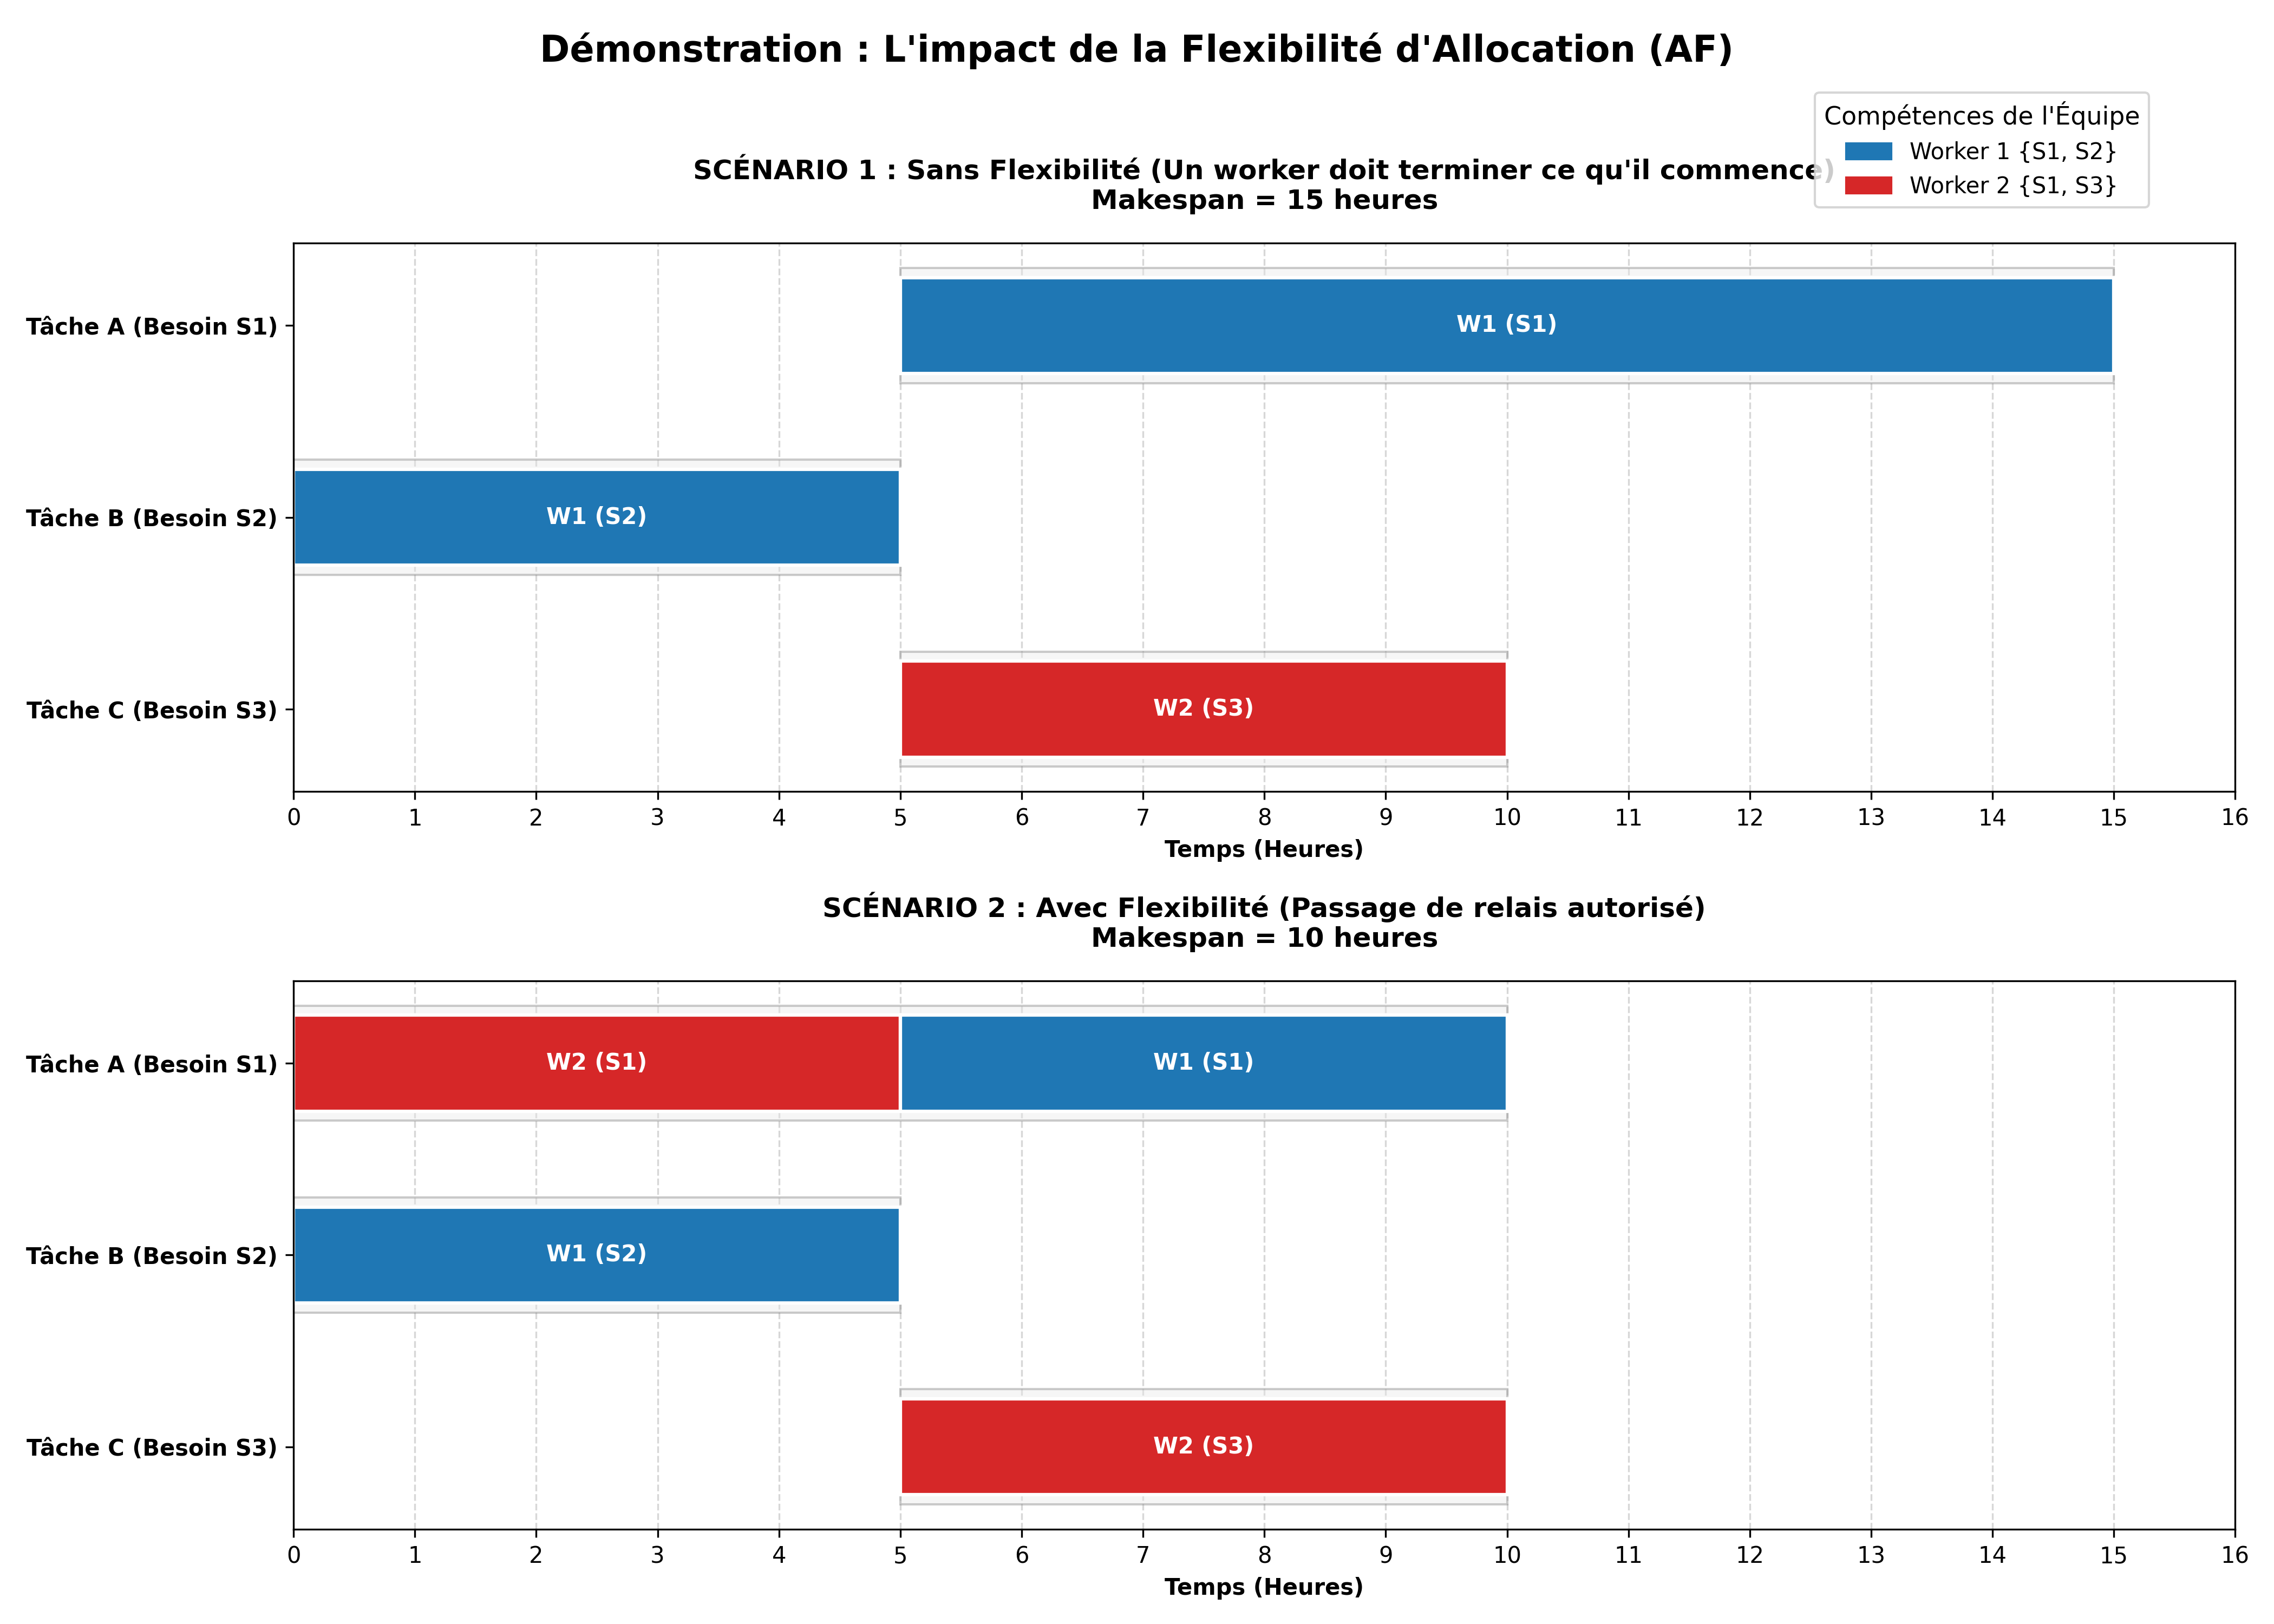
\includegraphics[width=0.9\textwidth]{imports/demonstration_af_relais.png}
    \caption{Illustration de l'impact de la flexibilité d'affectation (AF) sur le Makespan d'un projet}
    \label{fig:demonstration_af}
\end{figure}

\vbox{
Si cette flexibilité permet d'optimiser l'usage des ressources et de réduire le makespan, elle augmente la complexité du problème. Contrairement aux approches classiques où l'affectation est fixe pour toute la durée d'une tâche, la flexibilité impose de valider la faisabilité de l'affectation à chaque unité de temps. Cela génère une combinatoire importante, renforcée par des symétries d'affectation lorsque les opérateurs partagent des compétences identiques. Les solveurs peinent alors à élaguer l'arbre de recherche.
}

\bigskip

La littérature de la recherche opérationnelle s'est largement intéressée au problème classique d'or\-donnancement de projet sous contraintes de ressources (RCPSP). L'intégration de ressources multi-compéten\-ces, introduite par Bellenguez-Morineau et Néron \cite{bellenguez2007branch, bellenguez2008multi}, a suscité un intérêt croissant, comme le montre la revue de littérature de Snauwaert et Vincke \cite{snauwaert2023classification}. Les approches exactes traditionnelles reposent souvent sur la programmation linéaire en nombres entiers (MILP), étudiée par Almeida et al. \cite{almeida2019modeling}, mais ces formulations présentent des limites de passage à l'échelle lorsque l'horizon s'allonge. Pour y remédier, des approches basées sur la génération de colonnes (Branch-and-Price) ont été explorées \cite{correia2015modeling, montoya2014branch}. Parallèlement, la Programmation par Contraintes (CP) s'est imposée comme une alternative pour modéliser des contraintes complexes \cite{young2017constraint, polo2020mixed}. Néanmoins, ces modèles monolithiques atteignent leurs limites sur des instances de grande taille en raison de la combinatoire induite par la flexibilité. C'est pourquoi la recherche s'oriente vers des méthodes de décomposition hybrides. La Décomposition de Benders basée sur la Logique (LBBD), introduite par Hooker \cite{hooker2000logic, hooker2019logic} et analysée par Cire et al. \cite{cire2016logic}, apparaît comme l'une des méthodes les plus adaptées. Contrairement aux schémas de Benders classiques qui délèguent l'ordonnancement au sous-problème, certaines approches d'ordonnancement multi-compétences inversent ce schéma en résolvant l'ordonnancement global dans le problème maître en CP et l'affectation dans le sous-problème. Cette inversion, introduite par Yi-fan et al. \cite{yi2013new}, a été étendue par Juvin et al. \cite{juvin2026logic} pour modéliser la flexibilité d'affectation (AF) dans le cadre du MS-RCPSP-AF, permettant le remplacement des travailleurs au cours de l'exécution des tâches.
\bigskip


\subsectionnn{Annonce du plan}

Ce manuscrit est structuré en quatre chapitres principaux :

\bigskip
\noindent Le Chapitre 1 introduit la modélisation mathématique du problème sous forme de programme linéaire en nombres entiers (MILP). Cette approche permet de formaliser les contraintes d'affectation et de précédence, tout en mettant en évidence les limites de ce type de formulation.

\bigskip
\noindent Le Chapitre 2 explore la modélisation en Programmation par Contraintes (CP). Nous présentons la formulation classique par sous-intervalles unitaires, une variante reposant sur la contrainte de cardinalité globale (GCC) et des contraintes de bris de symétrie, en analysant leurs limites calculatoires respectives.

\bigskip
\noindent Le Chapitre 3 présente la Décomposition de Benders basée sur la Logique (LBBD). Ce chapitre détaille la génération de coupes logiques et le couplage entre un problème maître en CP pour l'ordonnancement global et un Sous-Problème d'affectation résolu par flot maximum.

\bigskip
\noindent Le Chapitre 4 présente l'évaluation expérimentale des approches sur les instances des bibliothèques MSPSP-InstLib et  MSLIB, confirmant la supériorité de la décomposition face à l'explosion combinatoire subie par les modélisations monolithiques. Enfin, un aperçu sur les perspectives de recherche conclut ce manuscrit.
\bigskip
